\chapter{Analyse du parcours universitaire des bacheliers (UCAD)}

\section{Introduction}

\section{Évolution des inscriptions à l'UCAD}

\subsection{Les inscrits des série STEG et G}

\begin{figure}[h]
\centering
\caption{Évolution des inscriptions à l'UCAD pour les séries STEG et G}
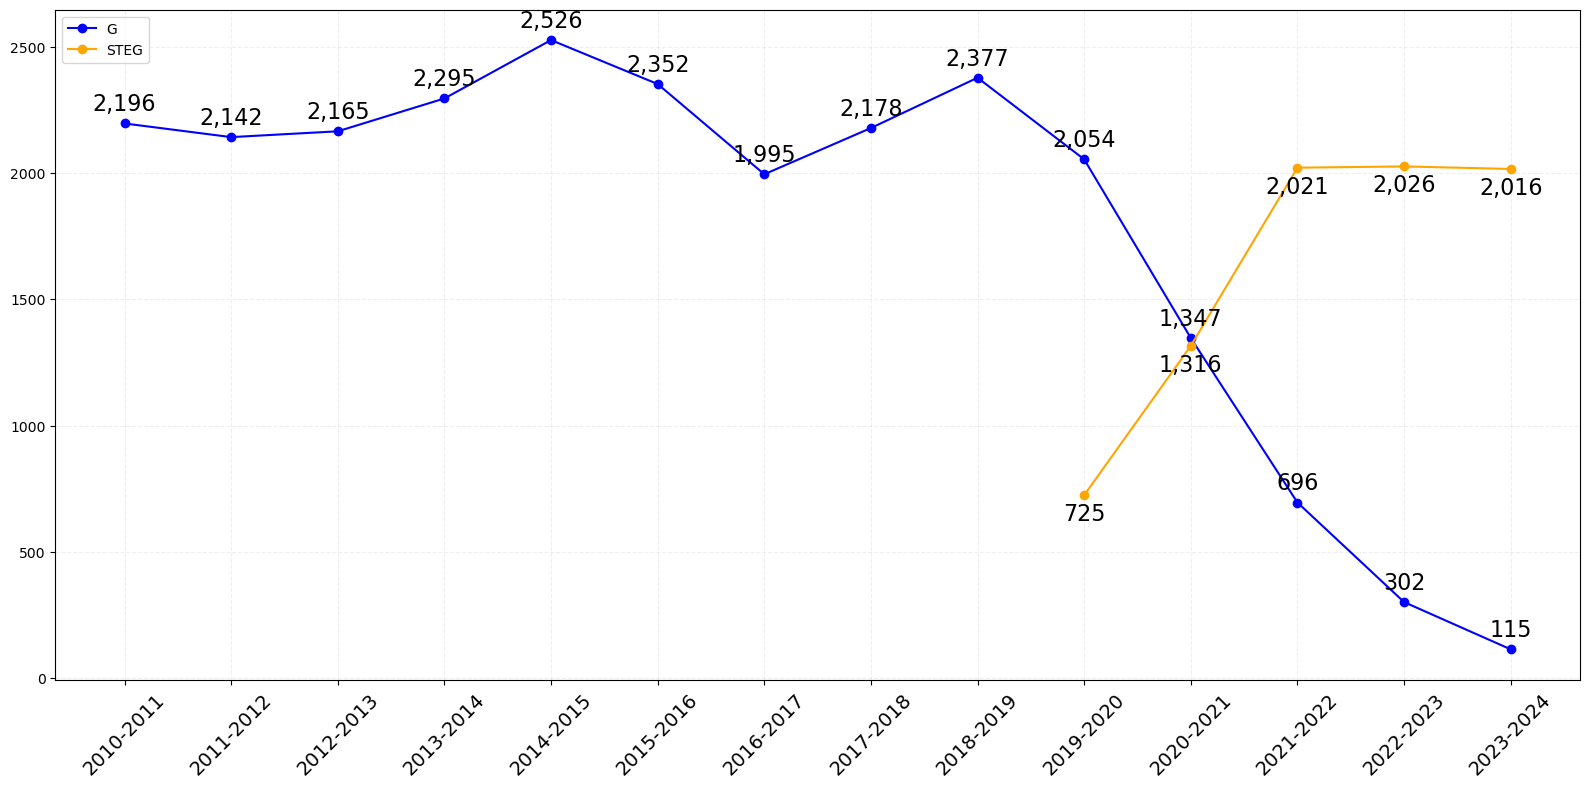
\includegraphics[width=1\textwidth]{figure/Inscrits_ucad_STEG.png}
\end{figure}

\newpage
\subsection{Les inscrits des séries Arables et Franco-Arabes}

\subsubsection{Série LA et LAR}

\begin{figure}[h]
\centering
\caption{Évolution des inscriptions à l'UCAD pour les séries LA et LAR}
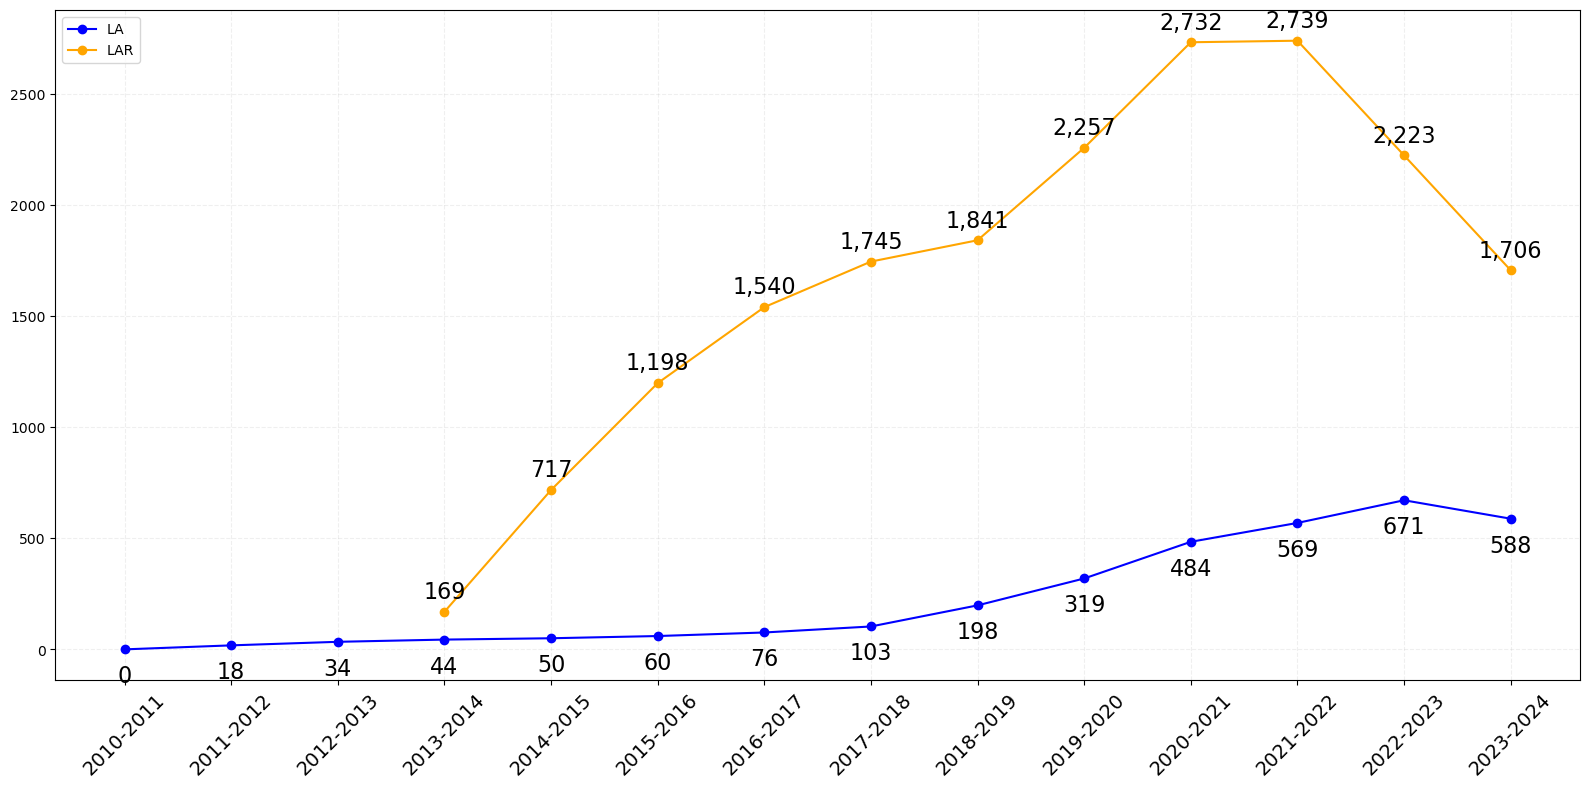
\includegraphics[width=1\textwidth]{figure/Inscrits_ucad_LA_LAR.png}
\end{figure}

\newpage
\subsubsection{Série S2A et S1A}

\begin{figure}[h]
\centering
\caption{Évolution des inscriptions à l'UCAD pour les séries S2A et S1A}
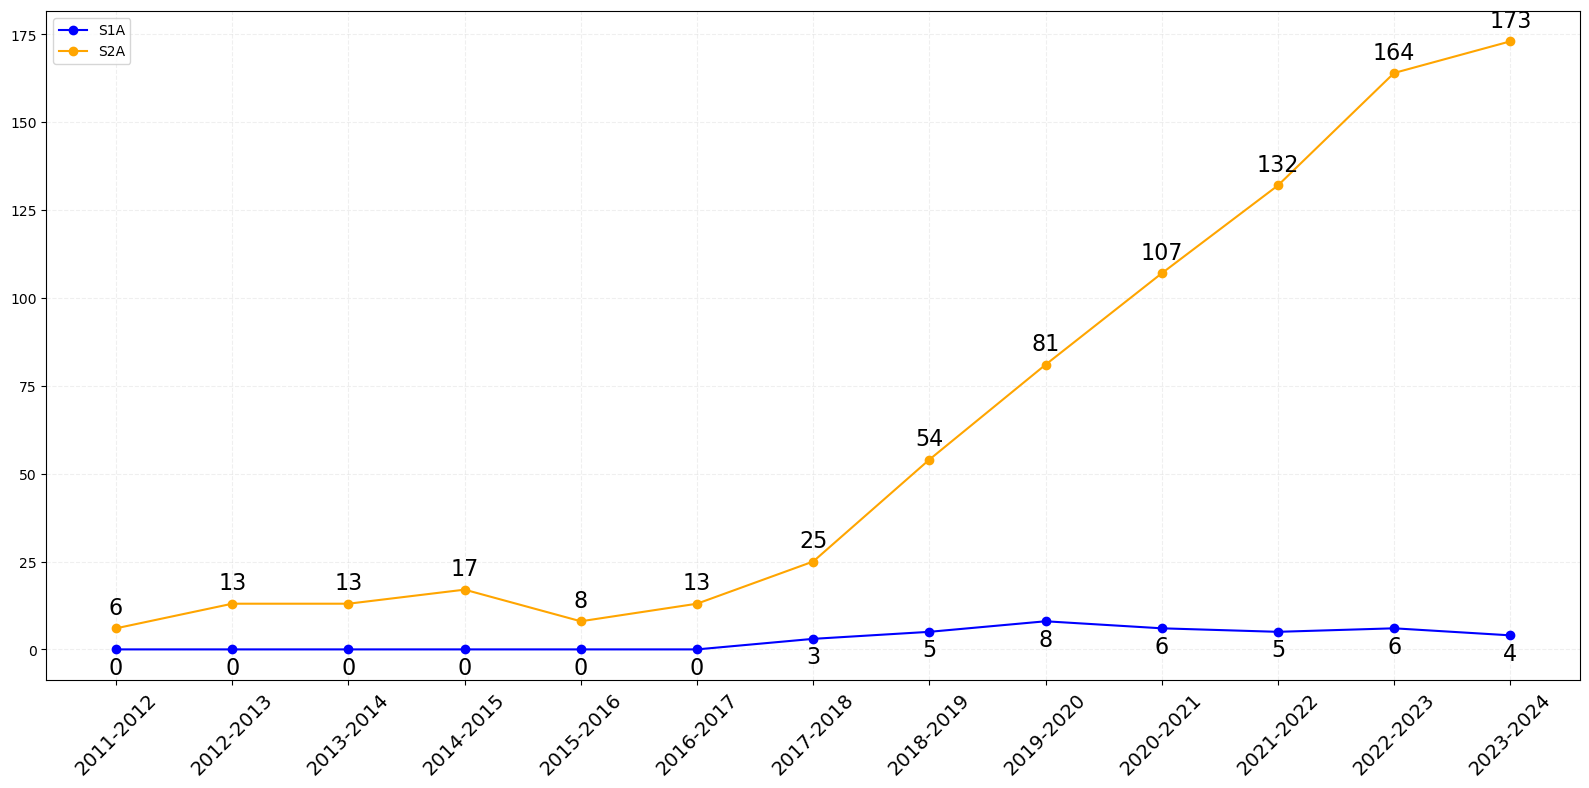
\includegraphics[width=1\textwidth]{figure/Inscrits_ucad_SA.png}
\end{figure}

\newpage
\section{Répartition des Inscrits par Établissement et Département}

\subsection{Série STEG et G}

\begin{figure}[h]
\centering
\caption{Évolution des inscriptions à l'UCAD pour les séries STEG et G (détail)}
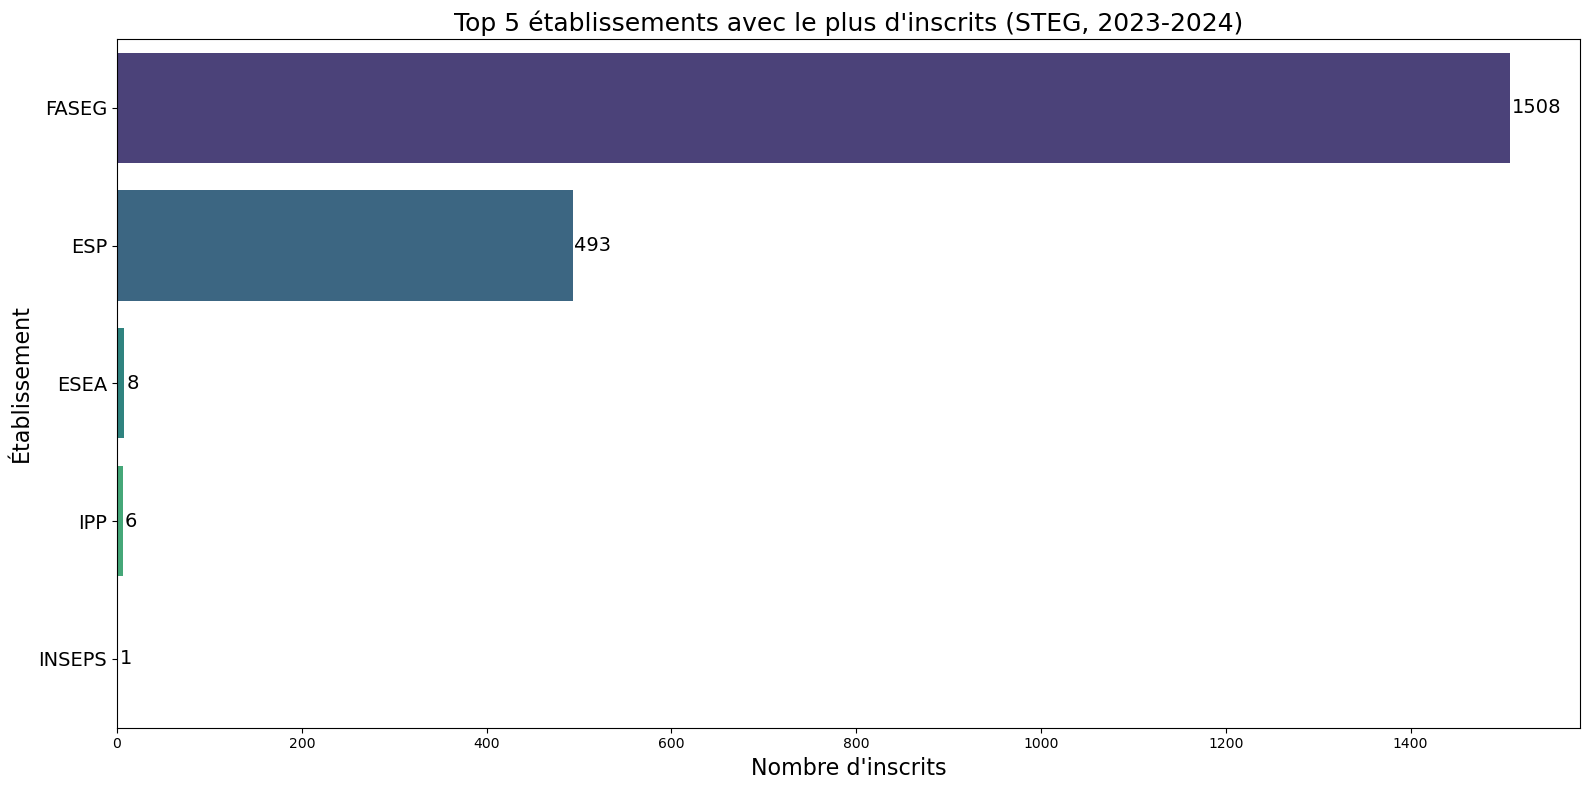
\includegraphics[width=1\textwidth]{figure/etab_STEG_2024.png}
\end{figure}

\begin{figure}[h]
\centering
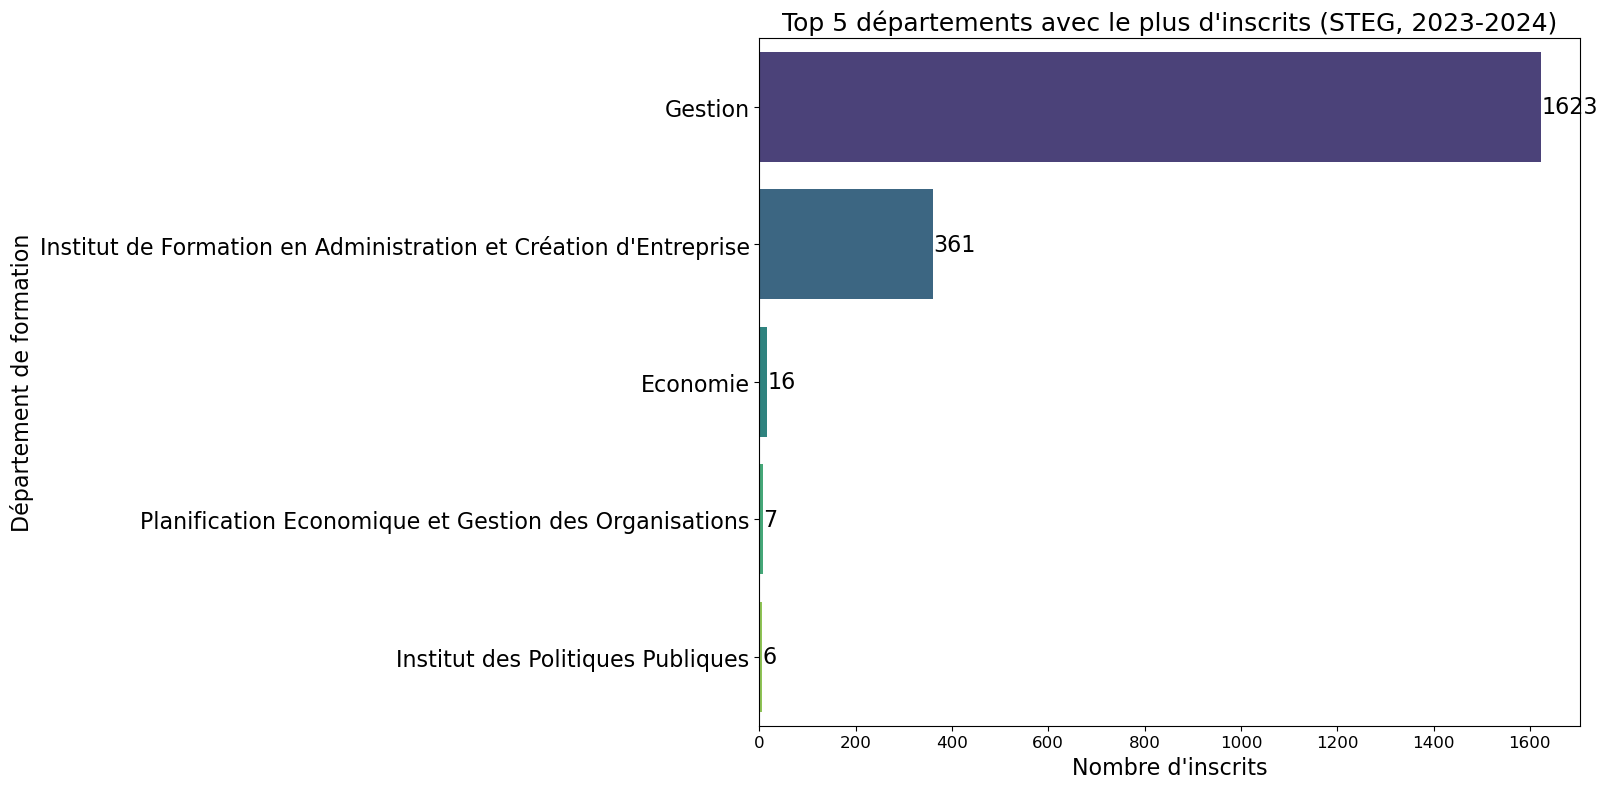
\includegraphics[width=1\textwidth]{figure/dep_STEG_2024.png}
\end{figure}

\newpage
\subsection{Série Arabes et Franco-Arabes}

\subsubsection{Série LA}
\begin{figure}[h]
\centering
\caption{Évolution des inscriptions à l'UCAD pour la série LA (détail)}
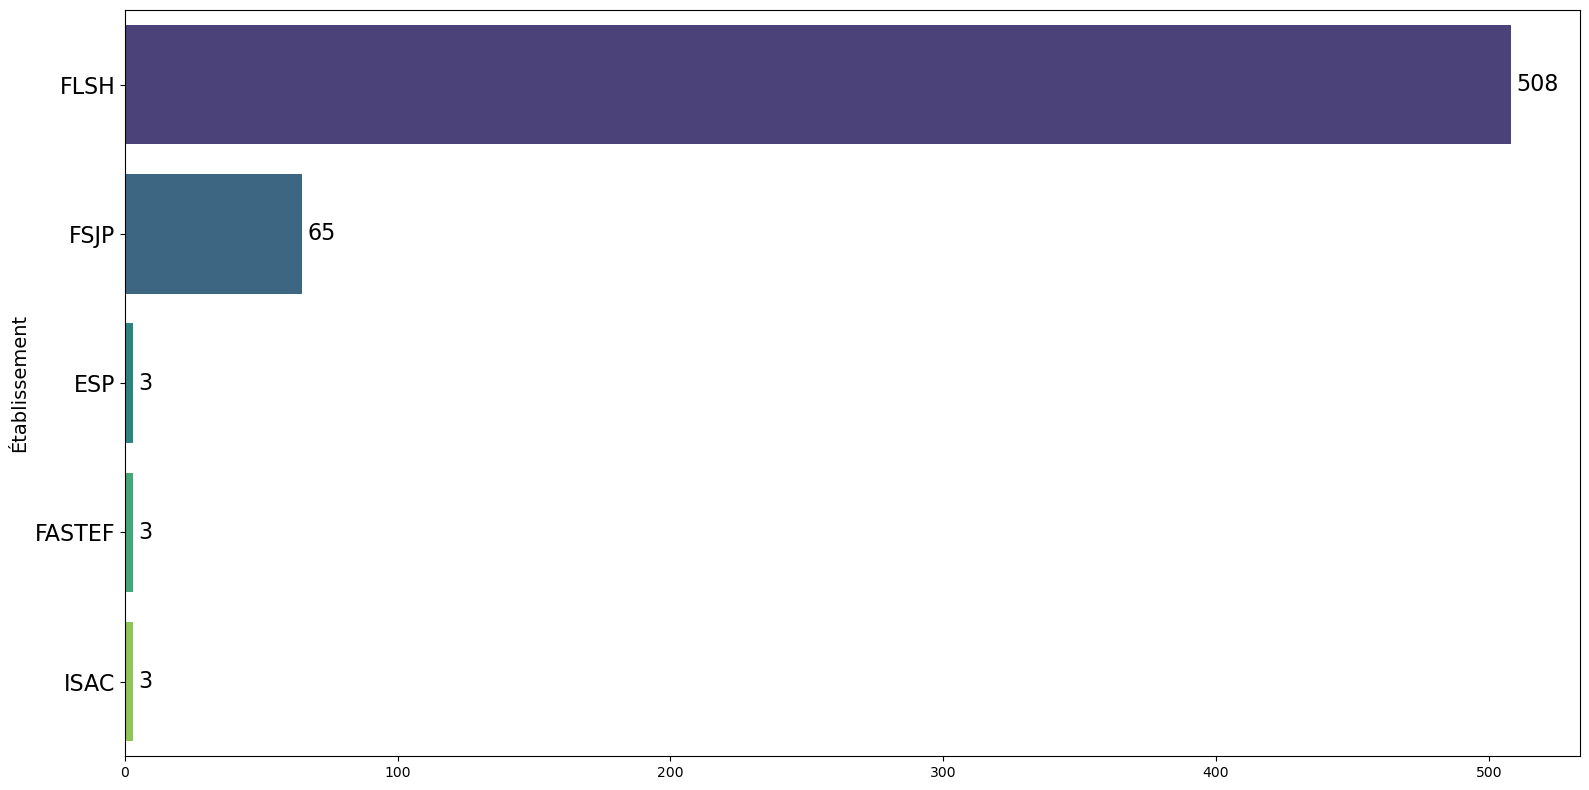
\includegraphics[width=1\textwidth]{figure/etab_LA_2024.png}
\end{figure}

\begin{figure}[h]
\centering
\caption{Répartition des inscriptions à l'UCAD pour la série LA par département}
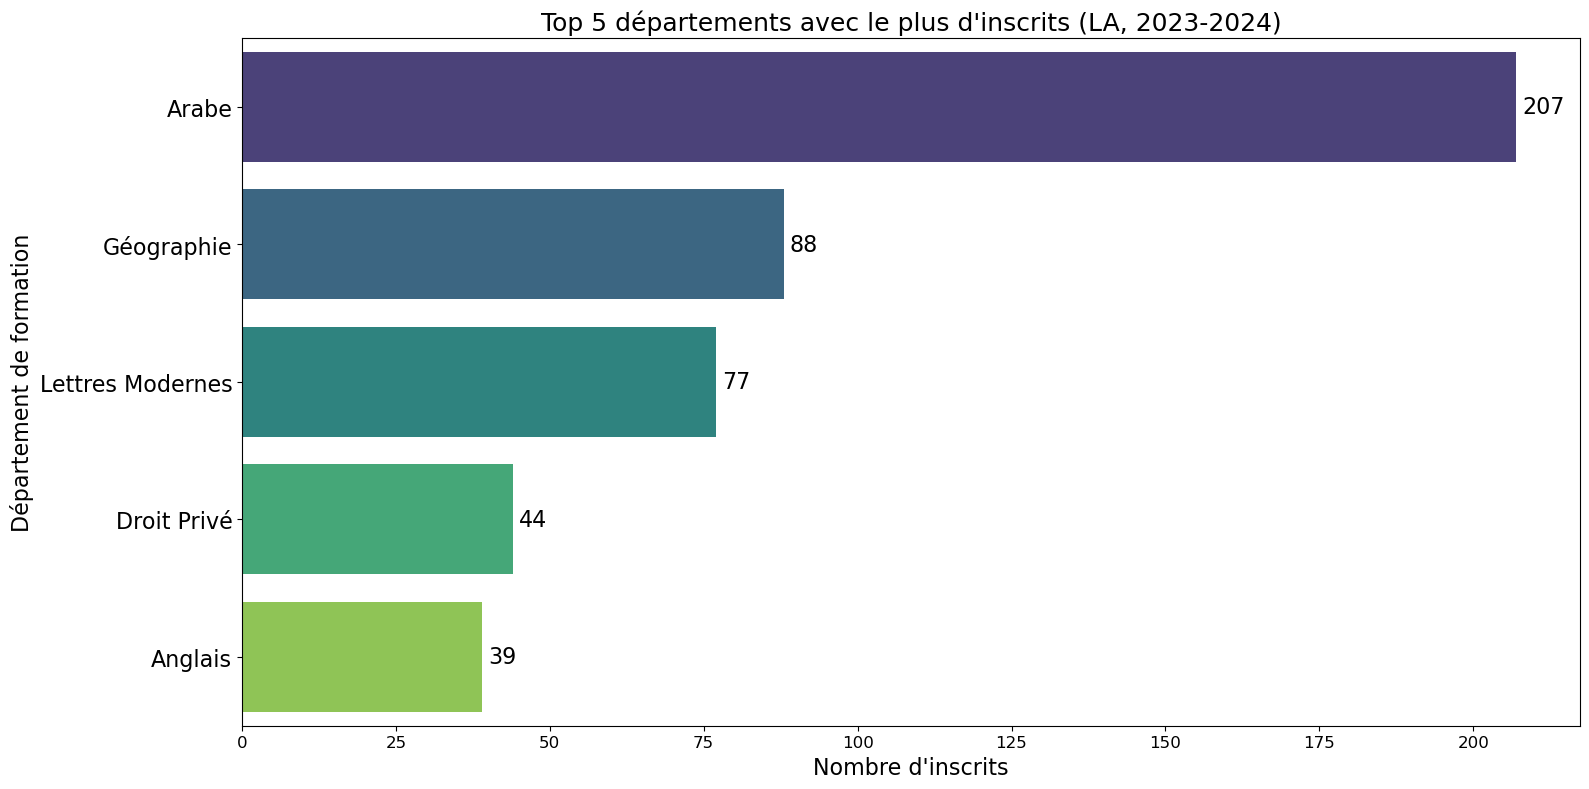
\includegraphics[width=1\textwidth]{figure/dep_LA_2024.png}
\end{figure}

\newpage
\subsubsection{Série LAR}

\begin{figure}[h]
\centering
\caption{Évolution des inscriptions à l'UCAD pour les séries LA et LAR (détail)}
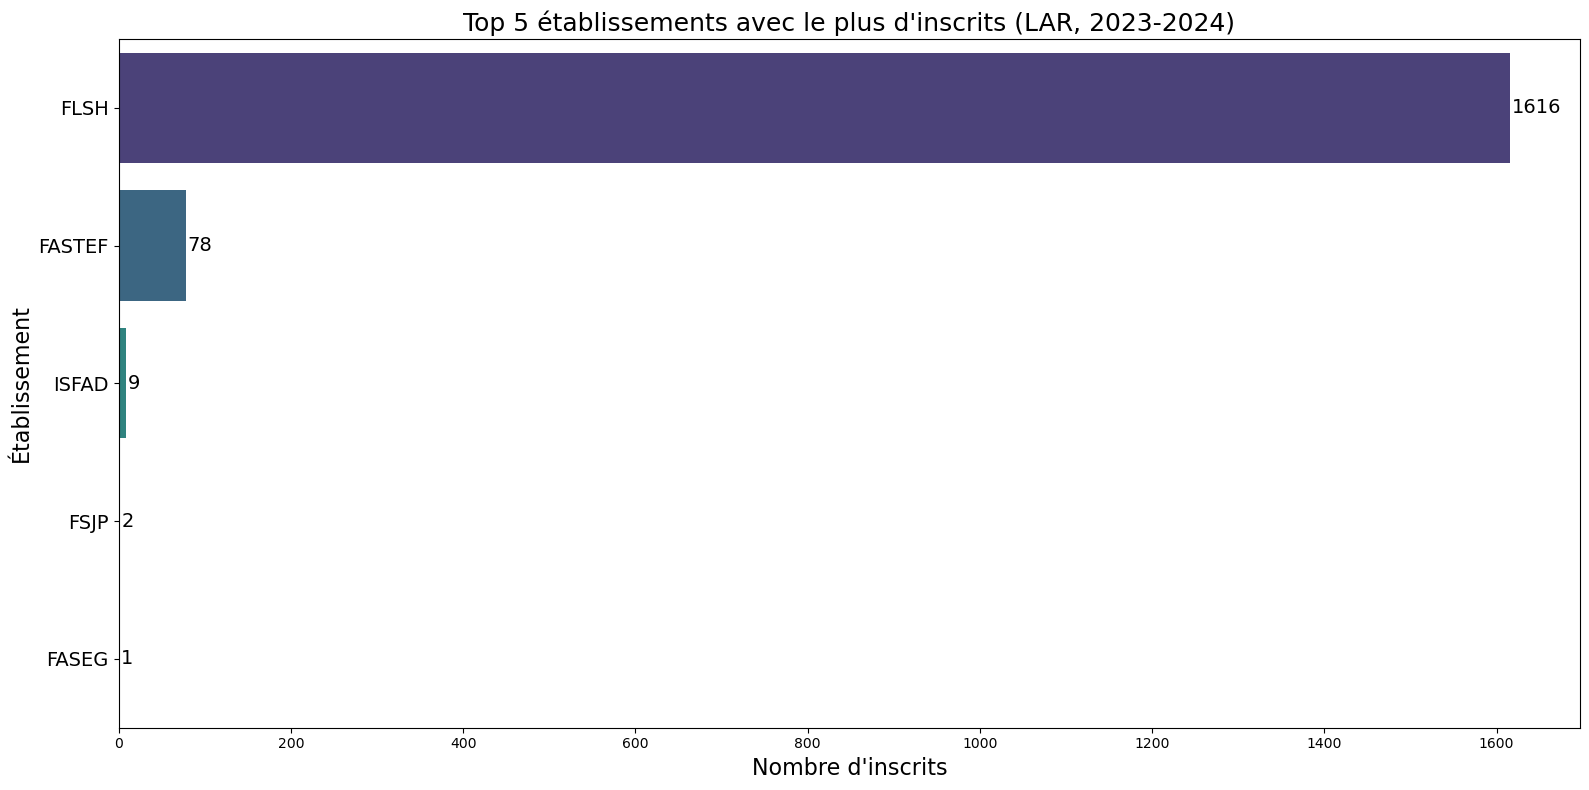
\includegraphics[width=1\textwidth]{figure/etab_LAR_2024.png}
\end{figure}

\begin{figure}[h]
\centering
\caption{Répartition des inscriptions à l'UCAD pour la série LAR par département}
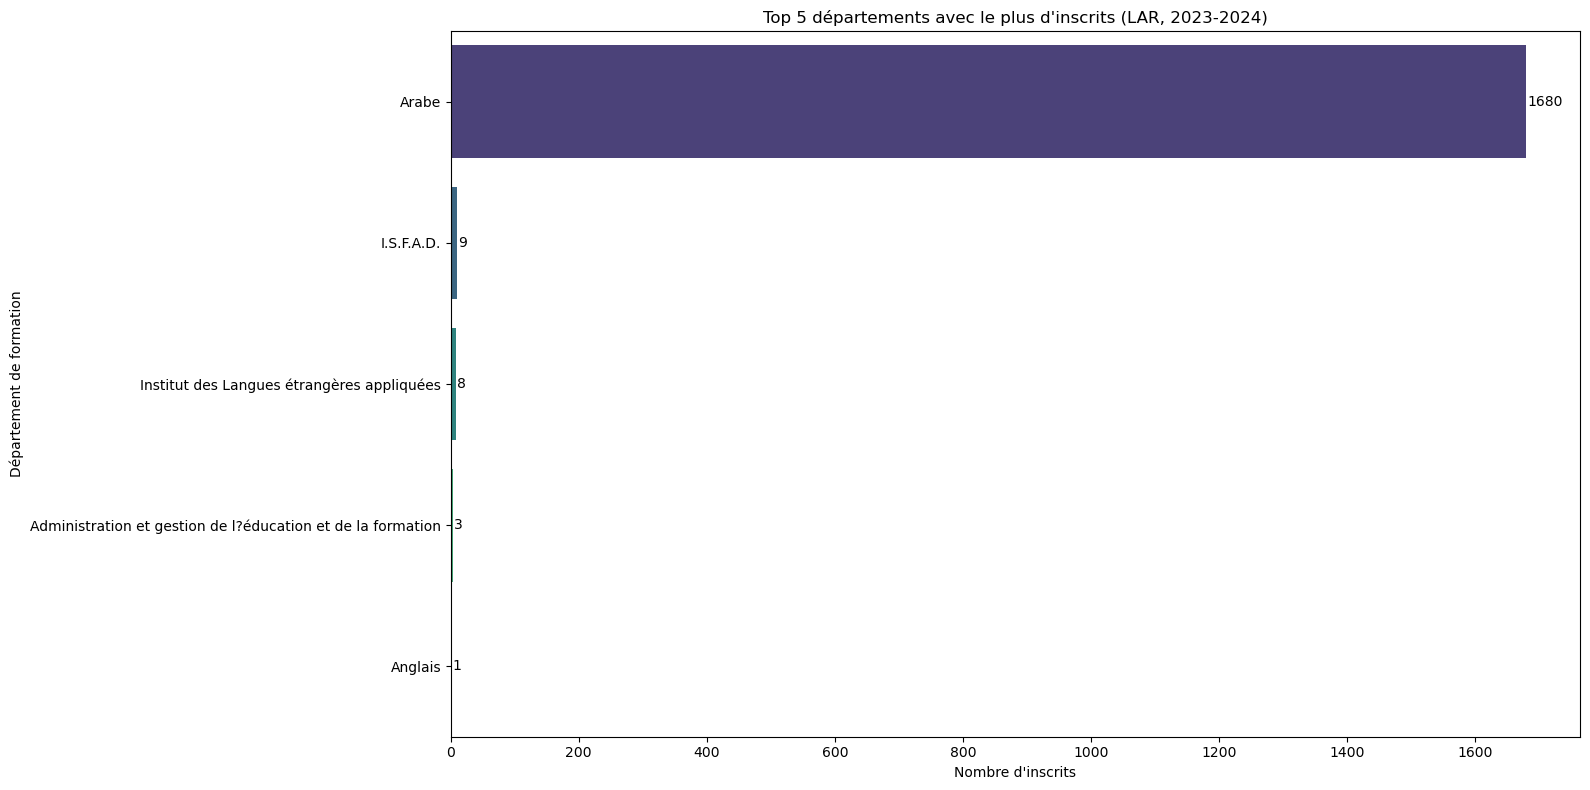
\includegraphics[width=1\textwidth]{figure/dep_LAR_2024.png}
\end{figure}

\newpage
\subsubsection{Série S2A}

\begin{figure}[h]
\centering
\caption{Évolution des inscriptions à l'UCAD pour la série S2A (détail)}
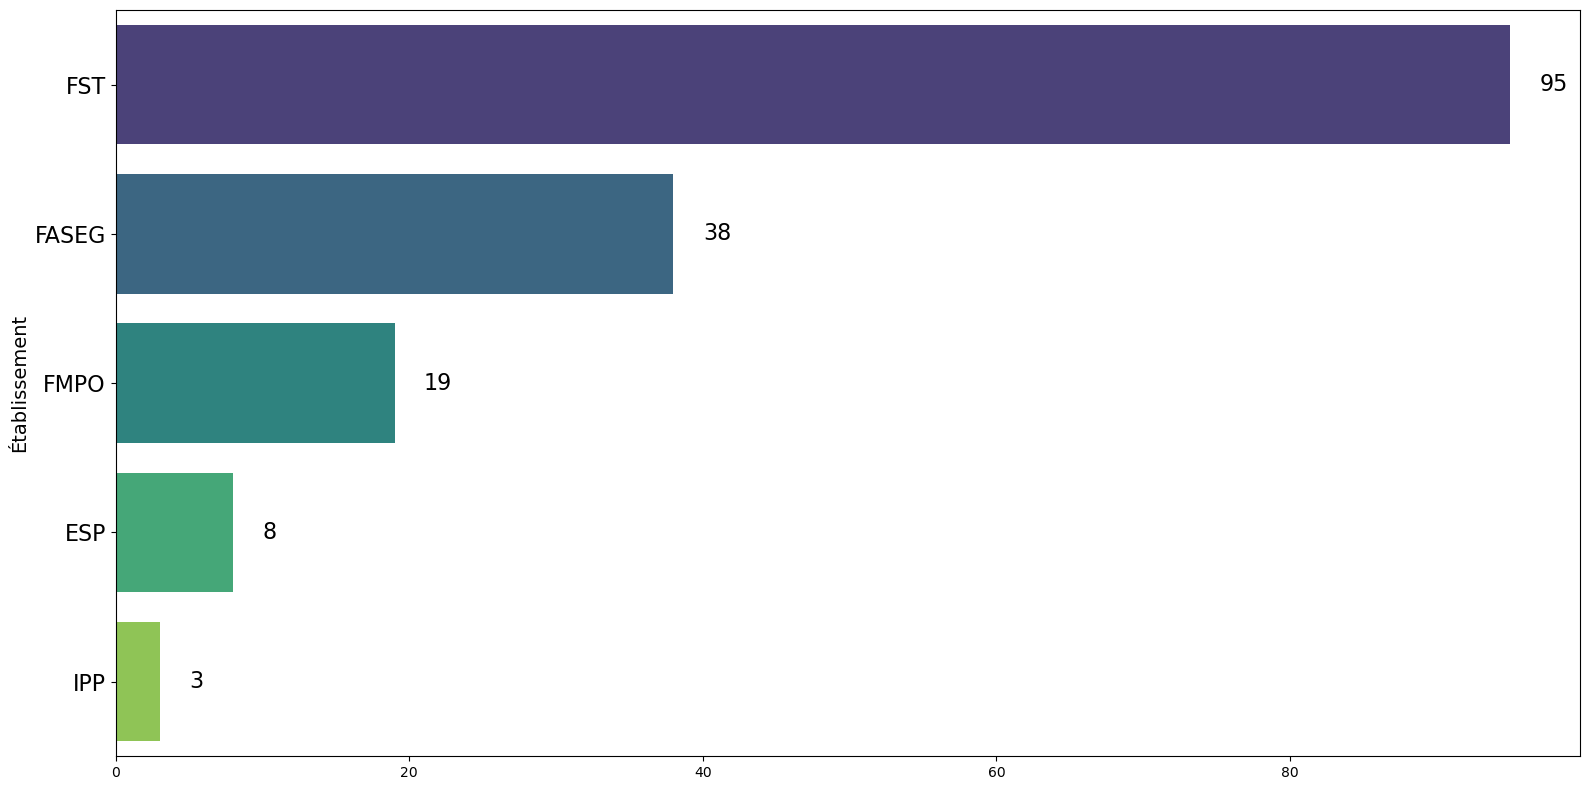
\includegraphics[width=1\textwidth]{figure/etab_S2A_2024.png}
\end{figure}

\begin{figure}[h]
\centering
\caption{Répartition des inscriptions à l'UCAD pour la série S2A par département}
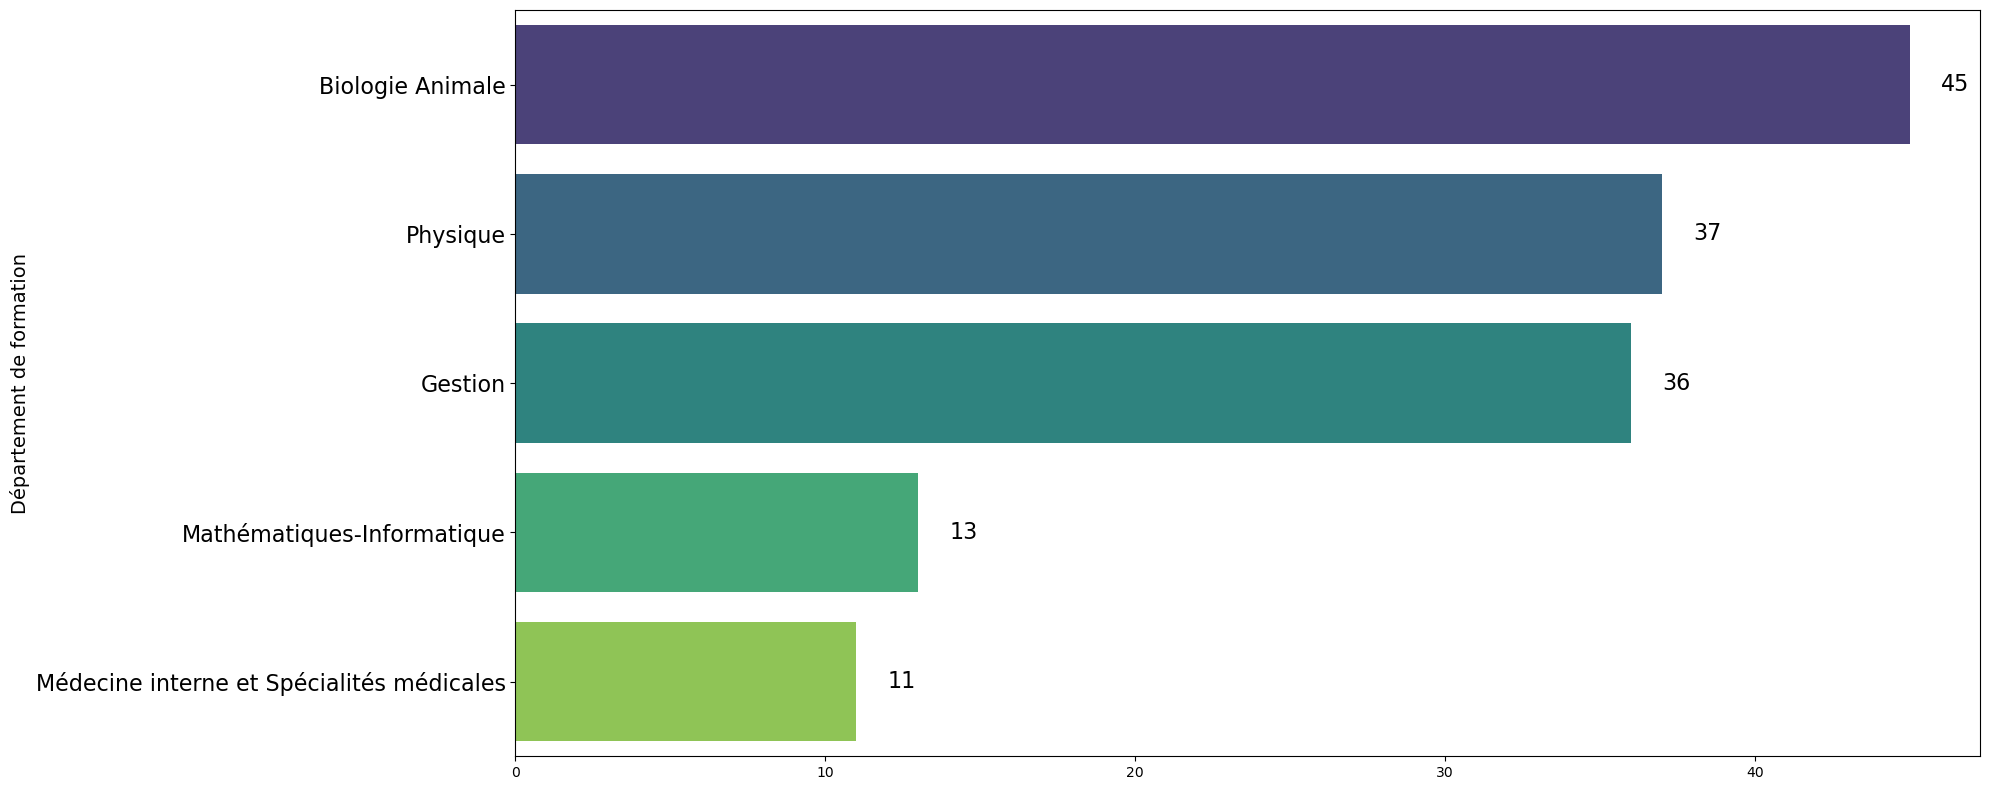
\includegraphics[width=1\textwidth]{figure/dep_S2A_2024.png}
\end{figure}

\newpage
\subsubsection{Série S1A}
\begin{figure}[h]
\centering
\caption{Évolution des inscriptions à l'UCAD pour la série S1A (détail)}
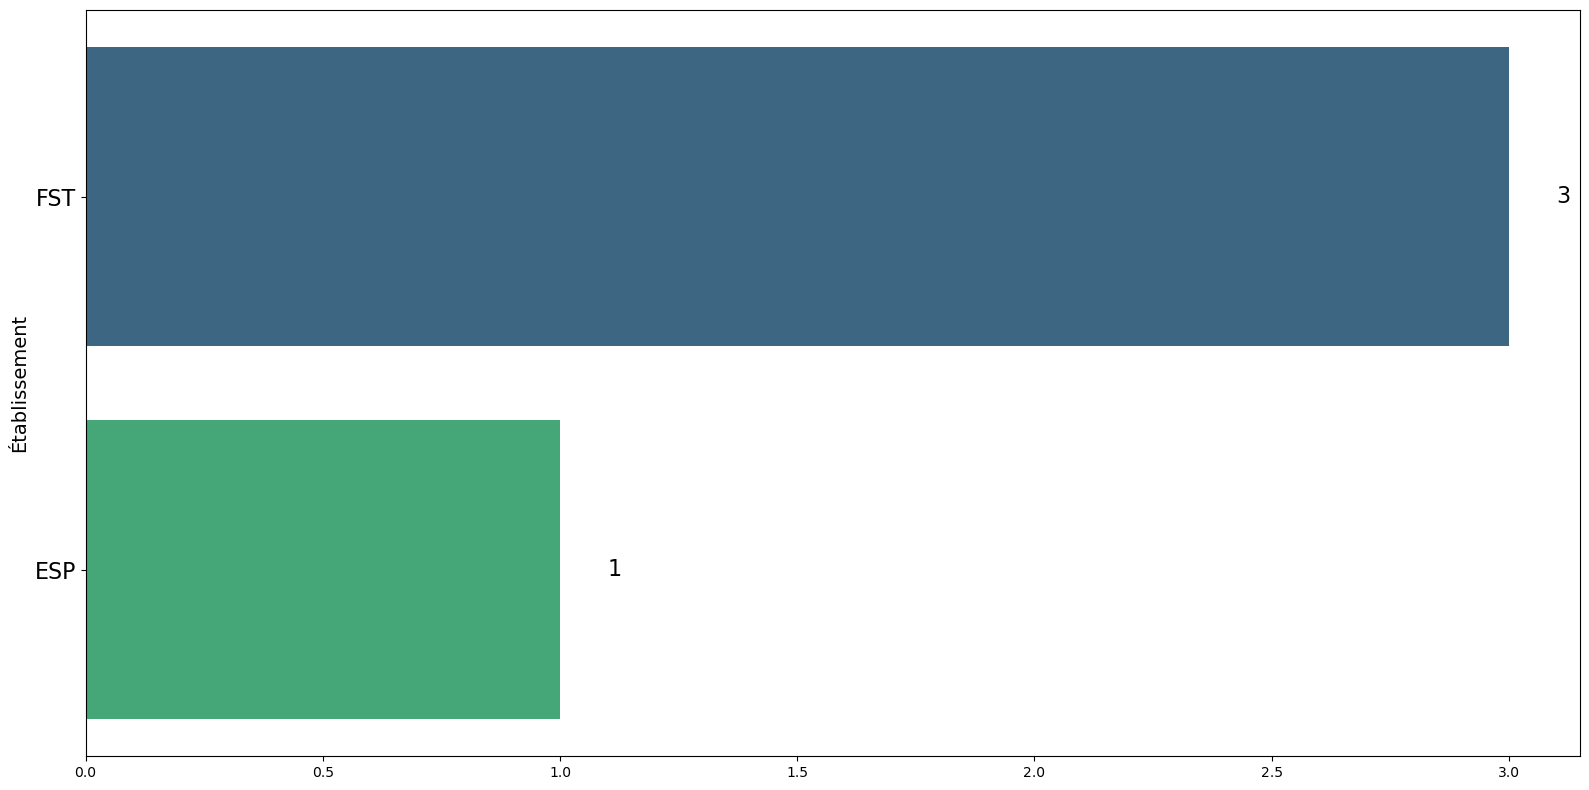
\includegraphics[width=1\textwidth]{figure/etab_S1A_2024.png}
\end{figure}

\begin{figure}[h]
\centering
\caption{Répartition des inscriptions à l'UCAD pour la série S1A par département}
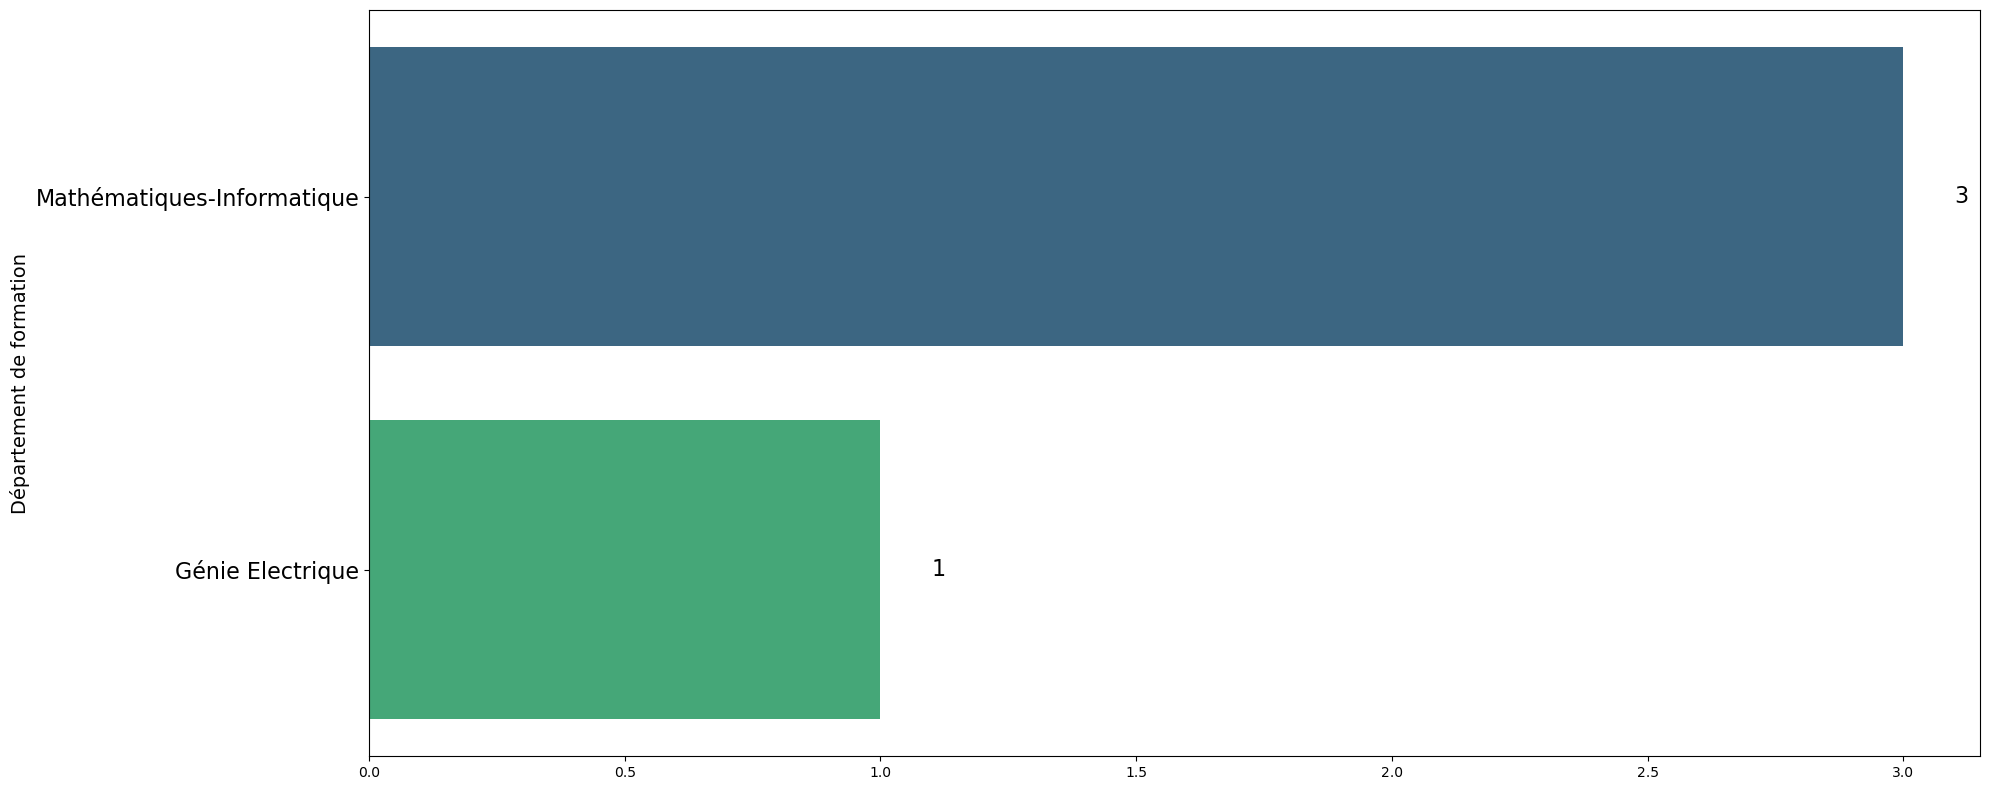
\includegraphics[width=1\textwidth]{figure/dep_S1A_2024.png}
\end{figure}

\newpage
\section{Analyse du parcours universitaire des bacheliers (suivi des cohortes)}

\section{Conclusion}